%%%%%%%%%%%%%%%%%%%%%%%%%%%%%%%%%%%%%%%%
% Classe do documento
%%%%%%%%%%%%%%%%%%%%%%%%%%%%%%%%%%%%%%%%

% Nós usamos a classe "unb-cic".  Deixe apenas uma das linhas
% abaixo não-comentada, dependendo se você for do bacharelado ou
% da licenciatura.

% Para tirar os comentários, é só mudar o comando para fazer nada.
\newcommand{\com}[1]{\textcolor{red}{#1}}%
\newcommand{\squote}{\textquotesingle}

\documentclass[mestrado]{unb-cic}



%%%%%%%%%%%%%%%%%%%%%%%%%%%%%%%%%%%%%%%%
% Pacotes importados
%%%%%%%%%%%%%%%%%%%%%%%%%%%%%%%%%%%%%%%%

\usepackage[UKenglish]{babel}
\usepackage[T1]{fontenc}
\usepackage{indentfirst}
\usepackage{natbib}
\usepackage{xcolor,graphicx,url}
\usepackage[utf8]{inputenc}
\usepackage{amsmath,amssymb,amsthm}
\usepackage{footnote}
%\usepackage{minipage}
\usepackage{tablefootnote} 
\usepackage{color}
\definecolor{darkgreen}{rgb}{0,1,0}
\usepackage{listings}
\lstset{% This applies to ALL lstlisting
    backgroundcolor=\color{yellow!10},%
    numbers=left, numberstyle=\tiny, stepnumber=1, numbersep=5pt%
    }%
% Add your keywords here, and have this in a separate file
% and include it in your preamble
% Applies only when you use it
\lstdefinestyle{ANTLR}{
    basicstyle=\small\ttfamily\color{magenta},%
    breaklines=true,%                                      allow line breaks
    moredelim=[s][\color{green!50!black}\ttfamily]{`}{'},% single quotes in green
    moredelim=*[s][\color{black}\ttfamily]{options}{\}},%  options in black (until trailing })
    commentstyle={\color{gray}\itshape},%                  gray italics for comments
    morecomment=[l]{//},%                                  define // comment
    emph={%
        STRING, color, icon, meta, name, private, var, grammar%                                            literal strings listed here
        },emphstyle={\color{blue}\ttfamily},%              and formatted in blue
    alsoletter={:,|,;},%
    morekeywords={:,|,;},%                                 define the special characters
    keywordstyle={\color{black}},%                         and format them in black
}
\definecolor{prismgreen}{rgb}{0, 0.5, 0} 
\lstdefinelanguage{Prism}{ % syntax highlight via font 
        basicstyle=\color{red}\scriptsize\ttfamily, % small true type font (like courier)
        breaklines=true,%                                      allow line breaks
        keywords={bool,C,ceil,const,ctmc,double,dtmc,endinit,endmodule,endrewards, endsystem,F,false,floor,formula,G,global,I,init,int,label,max,mdp,min, module,nondeterministic,P,Pmin,Pmax,prob,probabilistic,R,rate,rewards, Rmin,Rmax,S,stochastic,system,true,U,X},% 
        keywordstyle={\bfseries\color{black}},%
        numberstyle=\tiny\color{black},%
        comment=[l] {//}, morecomment=[s]{/*}{*/}, % single and multi-line 
        commentstyle= \color{prismgreen}, % dark green 
        tabsize=2, % tab treatment (going to be fixed in Prism) 
        captionpos=b, % put captions at the bottom 
        escapechar=@ % write LaTeX comments escaped by @ symbol 
} 

%define command \prism with one argument for inline printing of \prism code 
\newcommand{\prism}[1]{\lstinline[language=Prism,basicstyle=\small\ttfamily]|#1|}
\usepackage{enumerate}
\usepackage{booktabs}
\usepackage{tabularx}
%\usepackage{cleveref}
\usepackage{subcaption}
\usepackage{placeins}
\usepackage{url}
\usepackage{textcomp}


%%%%%%%%%%%%%%%%%%%%%%%%%%%%%%%%%%%%%%%%
% Cores dos links
%%%%%%%%%%%%%%%%%%%%%%%%%%%%%%%%%%%%%%%%

% Veja o arquivos cores.tex se quiser ver que outras cores estão
% pré-definidas.  Utilizando o comando \hypersetup abaixo nós
% evitamos aquelas caixas vermelhas feias em volta dos links.

\input{cores}
\hypersetup{
  colorlinks=true,
  linkcolor=DarkScarletRed,
  citecolor=DarkScarletRed,
  filecolor=DarkScarletRed,
  urlcolor= DarkScarletRed
}



%%%%%%%%%%%%%%%%%%%%%%%%%%%%%%%%%%%%%%%%
% Informações sobre a monografia
%%%%%%%%%%%%%%%%%%%%%%%%%%%%%%%%%%%%%%%%
\title{Dependability Verification for Runtime Goal Modelling}%

\orientador[a]{\prof \dr[a] Genaína Nunes Rodrigues}{CIC/UnB}
%\coorientador[a]{\prof[a] \dr[a] Coorientadora}{MAT/UnB}
\coordenador[a]{\prof[a] \dr[a] Alba Cristina Magalhaes Alves de Melo}{CIC/UnB}
\diamesano{30}{janeiro}{2015}%

\membrobanca{\prof[a] \dr[a] Vander Alves}{CIC/UnB}
\membrobanca{\prof \dr Luciano Baresi}{Politecnico di Milano}

\autor{Danilo F.}{Mendonça}
\CDU{004.4}

\palavraschave{\LaTeX, metodologia científica}
\keywords{\LaTeX, scientific method}



\graphicspath{{.}{img/}}%
\newcommand{\unbcic}{\texttt{UnB-CIC}}%
%%%%%%%%%%%%%%%%%%%%%%%%%%%%%%%%%%%%%%%%
% Texto
%%%%%%%%%%%%%%%%%%%%%%%%%%%%%%%%%%%%%%%%

\begin{document}
  \maketitle

  \begin{dedicatoria}

  \end{dedicatoria}

  \begin{agradecimentos}

  \end{agradecimentos}

\hyphenation{au-xi-li-ar}

  \begin{resumo}
  A static and stable operation environment is not a reality for many systems nowadays. Context variations impose many threats to systems safety, including the activation of context specific failures. Goal-oriented software-development methodologies adds the `why' to system requirements, i.e., the intentionality behind system goals and the means to meet then. Contexts may affect what requirements are needed, which alternatives are available and the quality of these alternatives, including dependability attributes. In order to allow a formal and probabilistic analysis of systems affected by context variation and elicited with Goal-Oriented Requirements Engineering (GORE) approach, we have proposed an extension to the TROPOS methodology to associate dependability constraints to goals and to provide a more precise and formal non-functional requirements (NFR) verification by translating a contextual goal model (CGM) annotated with a behavioural regular expression into a probabilistic model to be checked against properties defined with the Probabilistic Computation Tree Logic (PCTL). We evaluated the proposed TROPOS extension with a case study of a Mobile Personal Emergency Response System (MPERS).
  
%In this work, we propose the extension of the TROPOS methodology with a probabilistic model checking approach tailored for the verification of dependability requirements regarding multiple contexts of operation as part of the validation & verification phase of RE. 
  
  \end{resumo}

  \begin{abstract}
  	
  \end{abstract}
\hyphenation{a-tri-bu-tos}
  \tableofcontents
  \listoffigures
  \listoftables

\renewcommand{\appendixname}{Anexo}


  \textual
  
  \chapter{Introduction}\label{ch_introduction}%

\section{Problem Definition}

%praise
According to Lamsweerde, a poor requirements engineering (RE) is the major source of system failures. Lack of user involvement, requirements incompleteness, changing requirements, unrealistic expectations and unclear objectives are common causes~[AXEL]. Goal-oriented requirements engineering (GORE) has gained the attention of both academic and industrial practitioners due to its ability to systematically model the intentionality behind system requirements. More than just presenting the `what' and the `how', goal models also express the `why' of different requirements to exist. Its simple graphical notation allows non-technical stakeholders to take part in the analysis process and have a clear view of the system-to-be. Finally, automated model verification should avoid inconsistencies in the requirements specification.

% both strategically through higher level goals and operationally through lower level goals and tasks

In traditional GORE methodologies [GORE CA comparison], contribution  analysis are based on domain knowledge about the positive, neutral (implicit) or negative impact of a given system alternative to one or more system goals, generally a qualitative goal. By  comparing the overall contribution of two or more alternatives, a decision is made about which one should be adopted for the system-to-be. For instance, if one goal is to communicate with a remote user mobile, alternative means for the notification agent could be to send a SMS, an internet based message or a voice call. These alternatives may contribute with different values for qualitative goals such as `reliable delivery', `fast delivery', `convenient delivery', etc. 

The problem with this approach is threefold. First, it is based on domain knowledge information that may not exist or may not be precise and reliable. As a consequence, the decision of which alternative to use, either at design time or at runtime, may be biased and lead to unexpected violations - the selected alternative was actually unable to fulfil its qualitative goals. Second, it is limited to a static representation without any dynamic information that could be used to verify quality attributes that depend on system behaviour and its many nuances such as execution order, cardinality and execution priority. Finally, contribution links are deterministic. As such, the design decision based on contribution analysis is reduced to a simple sum comparison of the concurring alternatives with no support for probabilistic verification.

Additionally to the contribution analysis limitation, the context in which systems operate may not be static. Mobile and pervasive computing, among others, are examples of new computer paradigms for which the environment is not static, but dynamic. Battery, signals strength, components availability and the quality of physical resources and relevant information such as the user geographic location may vary through time, posing a new sort of challenge to the development of socio-technical systems based on these paradigms. The contextualization of the informations gathered at RE phase becomes imperative once its validity may be threatened by changing environment conditions~[Finkelstein, CGM]. Accordingly, any improvement of the GORE contribution analysis may have to consider multiple operational contexts.

%for these systems must also address the problem of multiple contexts of operation.

%The contextualization of an information means that its validity is not absolute in respect to the state of the world it relates to.

\section{Proposed Solution}

In order to provide a more solid and precise approach for the non-functional verification of different system alternatives and to improve the GORE contribution analysis, we propose the extension of the TROPOS goal-oriented software development methodology with a probabilistic model checking (PMC) approach that has already been explored and is supported by tools such as PRISM model checker[genaína PMC, PRISM]. The resulting verification model should represent activities that fulfils the root goal or any lower level goal and its elicited alternatives. This model should then be checked for properties that will provide estimations for the global or local non-functional requirements such as reliability, availability, performance and power consumption. 

The PMC technique used by this proposal requires a behaviour system specification. As the goal model proposed in TROPOS is static, no information regarding achievement/execution order, cardinality and priority of goals/tasks is available, except the activity diagram for the detailing of an agent's single capability behaviour and the sequence diagram for agents interaction. Nonetheless, this problem was tackled by Dalpiaz et al. with a regular expression language to express runtime information, e.g., how many times the same goal should be achieved and the execution order of different system tasks~[RGM]. We have used this proposal to fill the gap between the static goal model and its dynamic representation. Finally, this dynamic view of the goal model is translated to a probabilistic model following PMC technique. Our work uses the PRISM model checker and its language for this purpose and the Probabilistic Computation Tree Logic (PCTL) for property definition.

To address the problem of a dynamic context of operation, the context effects over goals, means and metrics should be parametrized to produce a formula that can check the system and its alternatives for different contexts. This verification, performed as part of the Validation \& Verification (VV) phase in RE, should anticipate (contextual) violations of non-functional requirements. Treating a detected violation at design time may correspond to actions such as making a different choice for underlying components used by this alternative's tasks, optimizing its behaviour specification or even the disposal of this alternative as a means to satisfy its goal if there is at least one other valid alternative. PMC technique also allows the identification of system alternatives with more influence on each metric through sensitive analysis. 

Runtime self-adaptation is beyond the scope of this work. However, based on the contextual analysis provided by the CGM and the enriched non-functional and dependability analysis provided by the verification of different alternatives using the PMC technique, it should not be difficult to extend the approach with the additional monitoring, planing and execution capabilities of a self-adaptation loop and have a self-adaptive architecture and mechanism reflected upon its runtime goal model requirements. These concerns should be addressed in future work.

%This space variability problem becomes more complex with the contextualization of goals, means and metrics. According to Bosh et al.[cite Bosh 2004], a high degree of variability allow the use of software in a broader range of contexts. Traditional GORE approaches are mostly used to the selection of which single alternative would exist in the system-to-be for some static context. A dynamic environment can result in contextual violations that can not be resolved just by configuration management. In these cases, a space variability may be required to keep the system properly running in different contexts.


%to a specific kind of goal called \textit{softgoal}. Softgoals are goals for which there is no clear-cut criteria. Often, they represent qualitative intentions of stakeholders, in contrast to the 

\section{Evaluation}

This proposal was evaluated with the application of the extended TROPOS methodology to the development of a Mobile Personal Emergency Response System (MPERS). This system may be seen as a body area network (BAN) with extended functionalities related to ubiquitous emergency response running in a mobile device [BAD]. Instead of a home or hospital static environment, the MPERS is conceived to allow patients with different health risk degrees to maintain mobility while they are monitored and assisted. If a medical emergency is detected, a geolocation feature should point out the location where the emergency response team must be addressed to. The MPERS features were based on real emergency response systems available at the industry and also at the BAN explored in previews work by Fernandes[Fernandes].

The evaluation process was focused in revealing the major benefits and limitations of the extended TROPOS proposal. Time to market is an important aspect for any software development methodology. Also, the soundness and precision of the proposed probabilistic verification is crucial and must be evaluated as they should not result in mislead decisions about which alternatives should be used by the system. Instead, they must anticipate any violation that could lead to a system failure, specially severe or catastrophic failures, giving analysts valuable information about where the system requirements and specification should be tailored and improved.

\section{Contributions Summary}

This section summarizes the contributions of this proposal.

%A seguir um resumo das con

\begin{enumerate}

\item A new contribution analysis approach for the TROPOS Goal-oriented software development methodology.

\item Inclusion of context effects over goals, means and metrics in the probabilistic model using appropriate constructs and parameters for each case.

\item Conversion rules between different decomposition and runtime constraints in a runtime goal model to a probabilistic model in PRISM language.

\item A parser implementation for the regular expression (regex) language used in runtime goal models with support for execution order, cardinality, alternative execution, optional execution and conditional execution. 

\item An automatic generation of the PRISM model representing activities from a runtime goal model annotated with the runtime regex and graphically modelled using the TAOM4E tool that supports TROPOS methodology.

\end{enumerate}

\section{Document Organization}

This dissertation is organized as follows. Chapter~\ref{ch_baseline} presents the base concepts of this work and the most important related works. Chapter~\ref{ch_problem} details the problem tackled by this proposal. Chapter~\ref{ch_proposal} presents the new extended TROPOS methodology, the rules for the translation between the contextual goal model and the probabilistic verification model, the parser for the runtime regex and finally the implementation approach for the automatic generation of the probabilistic model in PRISM language. Chapter~\ref{ch_evaluation} evaluates the proposal and describes its benefits and limitations. Finally, Chapter~\ref{ch_conclusion} concludes this work with final considerations about the current proposal, related proposals and our future work.
  \chapter{Baseline}\label{ch_baseline}%

\section{Goal-oriented Requirements Engineering}

Goal-oriented requirements engineering brings forward the intentionality behind system requirements. More than just presenting the \textit{what} and the \textit{how} of a system-to-be, it provides the justification for each requirement, that is, they also present the \textit{why}. Through a directed graph tree that begins with a root goal, goals are connected trough decomposition links. Higher level goals are related to strategical concerns, while lower level and specially leaf-goals are related to technical and operational features of the system. 

The purpose of a goal model is to structure the process of RE, including the elicitation of social needs and requirements, the actors involved in delivering functionality and resources, the decomposition of higher-level requirements into more granular and detailed requirements, the operationalization through means-end plan/task decomposition and finally the comparison between different alternatives for the system-to-be. A goal model is said to be valid and complete if it follows all its syntactic rules and if all system goals are either decomposed, delegated to other actors or fulfilled by operational system tasks. 

Three frameworks/methodologies, namely KAOS, i* and TROPOS, represent the foundations for the goal model analysis used by a variety of other proposals [KAOS, i*, TROPOS]. Despite some differences among their syntax, they all share a set of core concepts:
\medskip

\large{\underline{Entities}}

\begin{itemize}

\item \textbf{Actor:} an entity that has goals and can decide autonomously how to achieve them. They represent a physical, social or software agent.
\medskip

\item \textbf{Goal:} are actors' strategic interests. A goal with a clear-cut criteria for its satisfaction is called a hard goal. In opposition, softgoals has no clear-cut criteria for deciding whether they are satisfied or not and are usually associated to non-functional requirements of an actor.
\medskip

\item \textbf{Task:} an operational means to satisfy actors' goals.

\end{itemize}
\medskip

\large{\underline{Relations}}

\begin{itemize}

\item \textbf{AND/OR Decomposition:} a link that decomposes a goal/task into sub-goals/sub-tasks, meaning that all (at least one) decomposed goal(s)/task(s) must be satisfied/executed in order to satisfy its parent entity. 
\medskip

\item \textbf{Means-end:} a means to fulfil an actor's goal through the execution of an operational task by the same actor.
\medskip

\item \textbf{Contribution link:} a positive or negative contribution between a given goal/task to a softgoal. Contribution links are used for deciding between alternative goals/tasks at design time (contribution analysis).

\end{itemize}

\section{Contexts}

Context may be defined as the reification of the environment that surrounds the system operation~[FINKElSTEIN]. Contexts, as already stated, may not be static, but dynamic. An actor, that may be a system, has no control over its context of operation. Accordingly, an actor must be able to support different contexts of operation without violating its goals. Moreover, actors should be able to monitor the state of its surrounding environment and decide which alternative means will be used to fulfil its goals, as some may only be valid or optimized in specific contexts.

In GORE, dynamic contexts may affect what goals a system have to reach, the means available to meet them and also the quality achieved by each alternative[CGM]. Root goal and higher level strategical goals are not contextualized as they represent the main purpose of a system [Finkelstein]. As these goals are decomposed in more granular sub-goals, a context condition may dictate if the goal is required for that context, limiting `what' a system should do, or if it is adoptable, limiting the option of `how' to fulfil a required goal. Finally, a context may also dictate the positive, neutral or negative contribution of using some goal or task to another goal, usually a qualitative softgoal. This last effect is the main focus of this work, as it is related to the GORE contribution analysis that we aim to improve.
 

\section{Dependability Analysis}

The concept of dependability is related to dependence and trust as well as the ability of a system to avoid failures that are more frequent and more severe than certain threshold. According to Avizienis et al., dependability encompasses the following attributes~[AVIZIENIS]: 

\begin{itemize}

\item Availability: readiness for correct service.
\medskip

\item Reliability: continuity of correct service.

\item Integrity: absence of improper system alterations.
\medskip

\item Safety: absence of catastrophic consequences on the user(s) and the environment.
\medskip

\item Maintainability: ability to undergo modifications and repairs.
\medskip

\end{itemize}

%A holistic dependability specification has to include not only the software operation, but also the requirements for which that operation is meant. Requirements are an important factor to decide the acceptable frequency and severity of a software failure. Similarly, context is another factor in that decision. The frequency and the likelihood of failures are related to the dependability attributes of reliability, availability and integrity. Both likelihood and severity of failures are related to safety. 
%
%At early project phases, hazard resolution may involve simply getting more information about hazards or generating alternative design solutions~\cite{Leveson:1995}. In our work, we have used a qualitative means to analyse the dependability to be delivered by goals of a certain system taking into account contextual effects. Our approach improves the understanding of systems fault-causality effect and the identification of best approaches to reduce risk or even determine rates for safety or system level functional failure. Moreover, dependability requirement analysis cannot be accurately fulfilled without taking into account the context under which the system will operate.
%
%
%Avizienis et al \cite{Laprie2004} proposed a failure classification taxonomy with four viewpoints characterizing failures. In our approach, we use two categories: domain and consequence. We use the domain category to distinguish \textit{content} failures from \textit{timing} failures:
%
%\begin{itemize}
%
%\item{\textbf{Content failure}: When the content of the information delivered by a system task deviates from its specification}
%
%\item{\textbf{Timing failure}: When the time of arrival or the duration of the information delivered by some system task deviates from its specification}
%
%\end{itemize}
%
%The consequence of failures enables the definition of failures' severity. Two limiting levels are predefined and other intermediary levels could be defined for each case:
%
%\begin{itemize}
%
%\item{\textbf{Minor failure}: The harmful consequences of failures are limited or at most similar to the benefits provided by the correct operation of the system}
%
%\item{\textbf{Catastrophic failure}: The harmful consequences of failures are incommensurably higher than the benefits provided by correct operation of the system}
%
%\end{itemize}
%
%More details on the complete failure classification can be found in \cite{Laprie2004}. In our approach, a part of this taxonomy is used to guide the definition of the classes of failures severities and therefore the required level of dependability for different system goals. It also takes part in the identification of which dependability attribute is related to each contextual failure occurrence.  

\section{PRISM Probabilistic Model Checker}

The state based, probabilistic model checking technique used in this approach is supported by the PRISM model checker tool~[PRISM]. PRISM allows the modelling and analysis of systems which exhibit random or probabilistic behaviour. The decision of using PRISM as the probabilistic state based model checker was due to the number of successful case studies that have used this tool, indicating its maturity [PRISM CS], and also due to its rich environment that is able to represent different kinds of probabilistic models and their evaluations.

PRISM may be used for many different kinds of model evaluations depending on the abstraction level, the type of probabilistic model and the PCTL properties to be analysed. PRISM language offers a rich set of constructs that may represent system modules and components, among others architectural and design configurations. 

To evaluate the current proposal with the MPERS case study, we have used the a discrete-time Markov chain (DTMC) probabilistic model and focused on the verification of properties related to dependability, i.e., the reachability of the final success state of a set of goal model activities that represents: 

\begin{itemize}

\item if the set is composed of the minimum set of activities that satisfies the root goal: its global reliability;  

\item if the set is composed of the minimum set of activities that satisfies any lower-level goal: its local reliability.

\end{itemize}

It will be up to the analyst and stakeholders to define which type of probabilistic model and which PCTL properties must be analysed for each different system. Dependability attributes may be relevant for any sort of system, but are certainly important for systems with some criticality degree, i.e., for those whose failure could have severe or catastrophic consequences for the user(s) and for the environment.

  \chapter{Related Work}\label{ch_related_work}

\section{Contextual Goal Model}

The Contextual Goal Model (CGM)~[CGM] proposed the contextualization of required goals, adoptable means (goals/tasks) and contribution links values. The main benefit of this work is to enrich the original goal model with the contextualization of entities and relations affected by context variations and to provide a rationale for context analysis. In contrast, the main problem tackled by the current work is the verification of non-functional attributes that requires a more precise and formal approach instead of the existing contribution analysis that is based on analysts direct evaluation of the forward impact between goals/tasks and softgoals. 

In this regard, the CGM provided more realistic and precise contribution analysis contextualized by environment conditions, but did not change the nature of the contribution analysis process. Our work has benefited from the CGM conceptual model and has extended the non-functional GORE analysis with a context-dependent formal verification, i.e., that includes different context effects in the probabilistic model used by the PMC to estimate the values of required non-functional attributes of the system and provide a reliable decision criteria for the selection of concurring alternatives in the goal model before it is implemented.

\section{Awareness Requirements}

Souza et al.~[AwaReq] proposed the Awareness Requirements (AwReq) as a meta-requirement in a goal model, i.e., AwReq specify the success/failure rate and temporal constraints for other requirements in the model, including goals, softgoals, tasks and other AwReqs (*-meta-requirement). The purpose is to enrich the original goal model and provide clear-cut criteria for self-adaptation, as runtime AwReq violations should be addressed by corrective actions. AwReq are formalized by a temporal logic formula, namely the Object Constraints Logic with Temporal Message (OCLtm).

Despite its contribution to the specification of meta-requirements in the goal models, AwReq do not provide an approach to analyse and validate its meta-requirements before system implementation and monitoring. Original GORE contribution analysis could be used to define the impact of a given alternative to some attribute or value composing the AwReq. However, the paper focuses only on attributes that can be monitored by the system at runtime. In contrast, our approach relies on the improved contribution analysis, i.e., the model based verification of attributes through PMC technique that can be performed at design time and provide alternative design decision criteria. Moreover, a similar meta-requirement is used by our approach to define PCTL properties that must be checked by the PMC. These properties are also associated to system goals.

\section{Runtime Goal Model}

Despite the use of goal models to support the monitoring and adaptation functions at runtime, Dalpiaz et al. argued that these works are `using design artefacts for purposes they are not meant to, i.e., for reasoning about runtime system behaviour'. As such, they proposed a conceptual distinction between the static goal model, named Design Goal Models (DGM), and the Runtime Goal Model (RGM) that extend DGM with `additional state, behavioural and historical information about the fulfilment of goals'~[RGM].

The main purpose of the RGM approach is to provide the proper specification of behaviour information among system goals. RGM defines a class model, while the Instance Goal Model (IGM) provides the instance model that must conform to its class specification. IGM are useful to have an instance representation of the RGM provided by the monitoring of the activities involved in fulfilling system goals. If the monitored IGM violates the RGM, then a corrective action would have to take place. Again, our work has benefited from the conceptual contribution, this time by using the runtime regex language to have a behaviour specification for system goals and use it to generate the probabilistic model. In contrast, our work does not cover instance and monitoring aspects and focuses on the \&V phase of RE to anticipate any violation and for the selection of the most appropriate concurrent alternative elicited for the system.

\chapter{Proposal}\label{ch_proposal}

In the PMC technique adopted by this proposal, a behavioural specification, usually provided by UML activity and sequence diagrams, are manually converted to a probabilistic model in PRISM language. As a goal model goes from strategical to operational leaf-goals, and each leaf-goal describes a desired state reachable by either a delegation to other actor or by a operational task, then a behaviour specification as proposed by the RGM may be seen as an activity diagram and be used to generate a probabilistic model in PRISM language. This allows the model checking of the corresponding goal model as a set of activities for which temporal and other behaviour aspects are specified by the runtime regex of the RGM.
  \chapter{Modelling the Problem}\label{ch:motivation}

\section{Motivation}

%According to Lamsweerde, a poor requirements engineering (RE) is the major source of system failures. Lack of user involvement, requirements incompleteness, changing requirements, unrealistic expectations and unclear objectives are common causes~[AXEL].

Goal-oriented requirements engineering (GORE) has gained the attention of both academic and industrial practitioners due to its ability to systematically model the intentionality behind system requirements. More than just presenting the `what' and the `how', goal models also express the `why' of different requirements to exist. Its simple graphical notation allows non-technical stakeholders to take part in the analysis process and have a clear view of the system-to-be. Finally, automated model verification should avoid violations of the requirements specification.

TROPOS is a GORE methodology that also includes architectural and  detailed design phases for the development of socio-technical systems. Socio-technical systems provide and control a wide range of daily used services. Often, these systems are responsible for important and even critical requirements whose failures would cause undesirable or intolerable consequences. This requires developers to take dependability into consideration as a first class requirement.

In TROPOS, as in other GORE frameworks, there is no coupling to any specific verification approach for dependability attributes and other non-functional requirements. Contribution analysis is used for the comparison and selection of alternative design solutions based on how each alternative contribute to one or more system goals, usually qualitative softgoals. This approach, however, is not tailored for metrics depending on system behaviour, i.e., on the dynamic coordination of activities and components interactions. 

Probabilistic fault-forecasting aims to derive probabilistic estimates about measures related to the behaviour of a system in the presence of faults. Dependability benchmark enables the characterization of the dependability and security of a system and the comparison of alternative solutions according to one or several attributes~[AVIZIENIS~37]. This benchmark may be achieved by a probabilistic model checking technique coupled to the later phases of the TROPOS methodology, enabling the dependability benchmark of a goal model.

An important success factor for any software development methodology is a reduced overhead to the development effort, including domain knowledge and tools to support its process. PMC may significantly reduce the occurrence of system failures, but it also requires additional knowledge about its modelling language and verification steps. A goal model extended by behaviour specification overlaps with the UML activity diagram used by PMC.  Moreover, an automatic model generation for the PMC is desirable to reduce the know-how and effort for the verification of metrics for the system, justifying the implementation of this generator as an extension of a TROPOS modelling tool.

\section{Requirements}

Based on the identified gap of a formal verification of non-functional requirements in a goal-oriented requirements engineering approach, we defined the following requirements that must be addressed by our proposal:

\begin{enumerate}[R.1]

\item \textbf{Backward compatibility:} Extended TROPOS runtime regex and contextual notation added to the goal model must not modify the existing syntax and semantic of the original TROPOS methodology.

\item \textbf{Optionality:} The use of the probabilistic model checking as a formal verification approach of runtime goal models as an extended TROPOS methodology should be optional and not mandatory.
\medskip

\item \textbf{Model generation:} The probabilistic model representing the activities of runtime goal models should be automatically generated.
\medskip

\item \textbf{Tool integration:} The same development environment tool used for TROPOS modelling and analysis activities should be extended with the runtime regex, context notations and verification model generation.
\medskip

\item \textbf{Static syntax support:} The verification model should be coherent to the static goal model syntax for the AND/OR decomposition of goals/tasks and for the goal-task means-end relation.
\medskip

\item \textbf{Dynamic syntax support:} The verification model should be coherent to the runtime goal model regex including tasks sequential or interleaved execution order, cardinality as well as alternative, optional and conditional tasks execution.
\medskip

\item \textbf{Contextual syntax support:} The verification model should be coherent to the context effects over the activation of goals, the adoptability of sub-goals/tasks and over the individual quality metric of components. 

\end{enumerate}  
  \chapter{TROPOS Methodology with Probabilistic Requirements Verification}\label{ch_proposal}

This chapter describes the extended TROPOS methodology applied to the MPERS case study. Both TROPOS requirements analysis phases are fully presented, as long as the verification process that requires a behaviour specification and the additional contextual notation regarding context effects. Further details about the TROPOS methodology may be found in the reference literature~[TROPOS]. 

\section{TROPOS Requirements Engineering Phases}

\subsection{TROPOS Early Requirements Phase}

In Early Requirements phase, stakeholders are modelled as actors and their needs as goals. Each actor may be a depender or a dependee of a goal, task or resource dependency. In this phase, only the main system actor and the application domain stakeholders are analysed, leaving the detailed system analysis to later development phases.

The MPERS sytem and its social dependencies are presented by the actor model in Figure~\ref{fig:MPERS_ER}. System actors and social actors are displayed in different colors. Among the stakeholders, the emergency center represents a private or public organization interested in providing an emergency response service to patients. Patient and doctor represent, respectively, the assisted person and the medical responsible for defining and evolving the emergency detection rules as part of an evolutionary approach for personal emergency response. Finally, sensors retailer should provide the vital signs sensors required for monitoring.

\begin{figure*}[ht]
\centering
\includegraphics[width=1\textwidth]{imgs/MPERS_ER.png}
\caption{MPERS at TROPOS early requirements phase}
\label{fig:MPERS_ER}
\end{figure*}

From the diagram in Figure~\ref{fig:MPERS_ER} it is possible to have a first view of the MPERS system-to-be. Main goals are divided in detecting, notifying and checking an emergency. Also, the ability to update the emergency rules at runtime (RT) is the fourth and last mandatory goal (AND-decomposition) that fulfils the root `Patient is assisted' root goal. Functional system goals are strictly related to stakeholders functional and non-functional needs.

The yellow circle indicates that MPERS is a system actor. MPERS goals can be seen with a regex indicating its dynamic behaviour as part of the runtime goal model specification required by the proposal. This notation is a reflex of the late requirements phase, as the TAOM4E tool supporting TROPOS methodology shares unique entities and relations among different development phases. The regex syntax is enclosed by brackets to differentiate then from goal name. In future work, a specific modelling compartment should receive the values for the runtime regex.

\subsection{TROPOS Late Requirements Phase}

Later requirements phase concentrates the analysis in the system-to-be and its operational environment. The MPERS goal model occupies the most part of the diagram and each of its main goals are further decomposed through AND/OR decomposition. Also, means-end tasks defines how leaf-goals are fulfilled and the runtime regex across goals and tasks specifies dynamic properties of the system-to-be behaviour. Figure~\ref{fig:MPERS_LR} illustrates the late requirements diagram for the MPERS.

\begin{figure*}[h!]
\centering
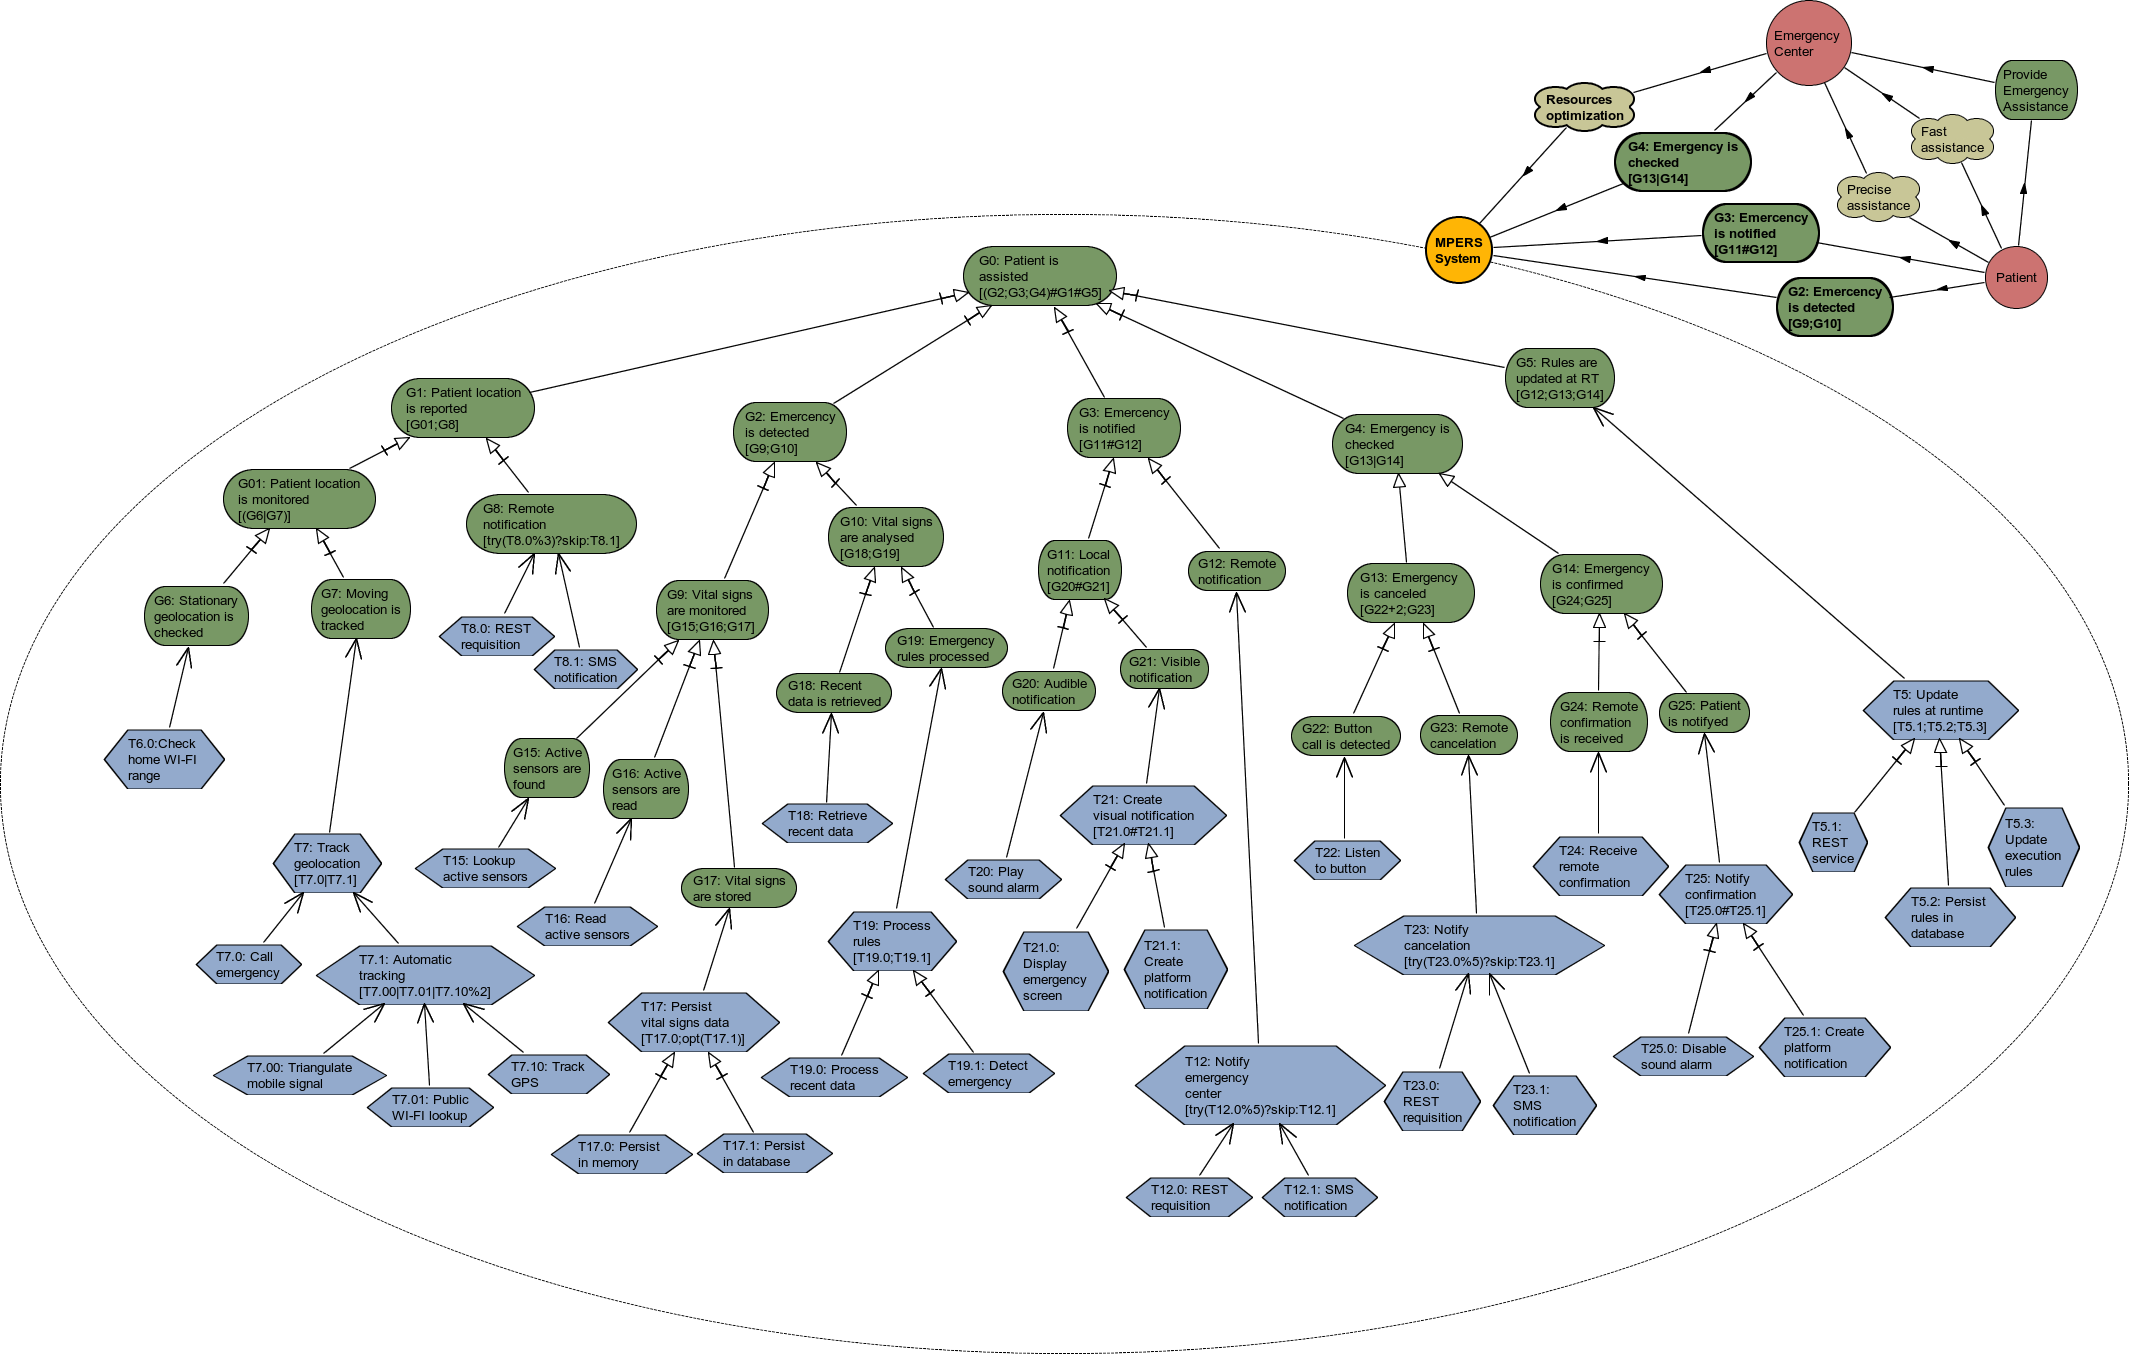
\includegraphics[width=1\textwidth]{imgs/MPERS_LR.png}
\caption{MPERS at TROPOS early requirements phase}
\label{fig:MPERS_LR}
\end{figure*}

At this point of the methodology, the system is represented as a monolithic actor and its goal model may be extended with the runtime specification. This extended model merges multiple views in the same diagram: strategical goals and operational tasks represent the requirements view for the system-to-be as well as the intentionality behind then, while the runtime specification provides a dynamic representation in terms of goal achievement  and task execution.

In this work, we have first explored the use of the PMC technique for the verification of dependability attributes in the system model of the late requirements phase. The idea is to initially evaluate the approach in a monolithic representation without the additional complexity of a multi-agent architecture. The evaluation involving later TROPOS phases should take place in future work. The remaining of this section will focus on the extended verification phase proposed by this work.

\section{TROPOS Extended Verification Phase}

To evaluate our verification approach with the MPERS case study, we have used a discrete-time Markov chain (DTMC) probabilistic model and focused on the verification of NFR related to dependability, i.e., NFR that are either direct attributes encompassed by dependability or that are related to one or more of these attributes.

\subsection{Runtime goal model}

In this section, further details about the runtime regex syntax and semantic will be explained as they are a central part of this proposal. In Figure~\ref{fig:MPERS_LR}, the runtime regex is already associated to system goals and tasks and Table~\ref{tab:RGM_REGEX} provides a textual description of each RGM notation with corresponding meaning in terms of what behaviour it specifies and also an example from the MPERS RGM. The formal and detailed description can be found in the reference publication~[RGM].

% Please add the following required packages to your document preamble:
% \usepackage{booktabs}
\begin{table}[h]\label{tab:RGM_REGEX}
{\renewcommand{\arraystretch}{1.5}
\begin{tabularx}{\textwidth}{@{}l|X|X@{}}
\toprule
\textbf{Expression} & \textbf{Meaning}                                                                   & \textbf{Example (MPERS)} \\ 
skip                & No action. Useful for conditional ternary expressions involving two elements.      & try(G10)?skip:G11        \\ 
E1;E2               & A goal/task E1 must be fulfilled/executed before E2.                               & G1;G2;G3                 \\ 
E1|E2               & Fulfillment/execution of goal/task E1 is alternative with respect to E2. & T9.1|T9.2                \\ 
opt(E)              & Fulfillment/execution of goal/task E is not mandatory.                             & opt(T17.2)               \\ 
E+n                 & Goal/task E must be fulfilled/executed n times, with n \textgreater 0.             & G22+2                    \\ 
try(E)?E1:E2        & If goal/task E succeeds, E1 must be fulfilled/executed; otherwise, E2.             & try(G10)?skip:G11        \\ 
E1\#E2              & Interleaved fulfillment/execution of goal/task E1 and E2.                          & G8\#G9                   \\ 
E\#n                & Interleaved fulfillment/execution of n instances of E, with n \textgreater 0.      & -                        \\ \bottomrule
\end{tabularx}
}
\caption{Description of RGM textual notations used by the proposal.}
\end{table}

\subsection{RGM-UML activity diagram comparison}

A similar specification could be provided by an UML activity diagram with activities as leaf-tasks of the goal model. However, activity diagrams have an homogeneous granularity level and do not clearly correlate behaviour to the requirements they are meant to satisfy. In contrast to the RGM, activity diagrams denote behaviour through graphical symbols, while the RGM mixes the original goal model notation with a runtime regex. This simple notation increases the utility of a goal model diagram. Figure~\ref{fig:MPERS_UMLAD} presents an activity diagram corresponding to the MPERS RGM. 

\begin{figure*}[h!]
\centering
\includegraphics[width=1\textwidth]{imgs/MPERS_UMLAD.png}
\caption{MPERS tasks represented by a UML activity diagram}
\label{fig:MPERS_UMLAD}
\end{figure*}

Among its limitations, RGM does not express that an emergency has to be confirmed after a time or signal event as the UML activity diagram does. Both necessary and sufficient conditions for the triggering and fulfilment of goals, tasks and dependencies are provided by Formal TROPOS language.  Still, sequential, parallel, alternative, optional and conditional execution flows as long as multiple executions of the same task can be expressed by the RGM, providing a rich behaviour specification that could be checked for non-functional requirements such as dependability attributes.

The idea of a runtime goal model is not to replace the activity diagrams, but to empower the goal model with a clear runtime syntax that could be used for 
documentation, communication and for conformance verification at both design time and during system execution - as it was originally proposed~[RGM]. Depending on the complexity of the behaviour specification, a more robust runtime syntax would have to be employed or a standard UML behaviour diagram such as activity and sequence diagrams would have to complement the goal model.

\subsection{Non-functional requirements specification}

The TROPOS goal model also provides rationale for NFR analysis either via softgoals or qualitative hard goals. As a benefit, the existence of one NFR may be justified by its relation to another NFR. Figure~\ref{fig:MPERS_NFR} presents the dependability NFRs for the MPERS system actor:

\begin{figure*}[h!]
\centering
\includegraphics[width=0.6\textwidth]{imgs/MPERS_NFR.png}
\caption{MPERS non-functional requirements.}
\label{fig:MPERS_NFR}
\end{figure*}

%Intersting for motivation!
Some dependability attributes, similarly to the Awareness Requirements by Souza et al.~[AWREQ], define metrics over other requirements. These meta-requirements are not directly fulfilled by system functionalities like `emergency awareness' is fulfilled by `notify emergency' or `confidentiality' could be fulfilled by `user authentication', but by how these functionalities will perform. Reliability, for instance, is inversely proportional to the likelihood of failures. Thus, the reliability metric depends on the probability of system functionalities to fail. Conformity to these metrics is not implicit in the model, it requires some verification technique.

Each requirement in a goal model must come from another requirement through decomposition, means-end or contribution links, or it must be directly mapped to a stakeholder need through dependency links. Emergency center attended the patient's needs by providing and maintaining the MPERS system itself and by assuring other NFR for the system. Availability and reliability were selected as metrics over the system execution (meta-requirement), while maintainability is partially satisfied by the MPERS ability to update emergency rules at runtime and by other aspects that, for the sake of simplicity, we will omit in this evaluation.

It is not an easy task to define the exact constraint to these metrics. For instance, an analyst or a reliability engineer should be aware of what does it mean for a system to be 99.999\% reliable, as this level may not be achieved by any alternative solution and must be coherent to the system criticality - a catastrophic failure should be avoided by all means. In some cases, the system will have to comply to some industry standards or contract based constraints. Table~\ref{tab:MPERS_NFR_C} summarizes each quantitative NFR for MPERS.
\medskip

% Please add the following required packages to your document preamble:
% \usepackage{booktabs}
\begin{table}[h]\label{tab:MPERS_NFR_C}
{\renewcommand{\arraystretch}{1.5}
\begin{tabularx}{\textwidth}{@{}XXX@{}}
\toprule
\textbf{NFR}               & \textbf{Constraint} & \textbf{Target}        \\ \midrule
\textbf{Reliability}       & 99.8\%            & \textbf{G1} \\
\textbf{Power consumption} & 100 p.u.            & \textbf{G2}          \\ \bottomrule
\end{tabularx}
}
\caption{Non-functional metrics for the MPERS system.}
\end{table}

%softgoals of `continuous assistance' and `correct assistance'

As indicated by the \textit{Target} column, each NFR constraint may be associated to a root level goal or to any of its subgoals. The corresponding probabilistic verification based on the execution of a set of system tasks in the RGM is defined as:

\begin{itemize}

\item \textit{Global}, if the activities set is a minimum set composed of the tasks that satisfies the chain of subgoals up to the root goal Groot, in this case identified as G1.
\medskip

\item \textit{Local}, if the activities set is a minimum set composed of tasks that satisfies the chain of subgoals up to a goal Gx, where Gx != Groot.
\medskip

\end{itemize}

%put here the formal definition of the root goal, subgoals, activity set, turple, etc

Other MPERS NFR are `emergency awareness' and `resources optimization'. These softgoals are addressed by system functionalities. The former receives a full contribution (double positive sign) from goal `emergency is notified', meaning it is fully satisfied by this goal. The later is just assumed to be partially satisfied by the `emergency is checked' functional goal.

\subsection{Non-functional requirements verification}


%NOT HERE!
The probabilistic verification of systems with variability is not a novelty by itself. Many proposals have addressed this problem in the context of Dynamic Software Product Lines (DSPL), some of then using the PMC technique~[Vini, Paula, Who Else?]. In DSPL, optional and alternative features may be activated or deactivated at runtime. A family based verification of one or multiple NFRs, also called qualitative goals, indicates what combinations are valid or which combination is optimal.

This section will describe the application of a PMC technique to verify the conformance of the RGM to defined non-functional constraints and also to solve the variability problem at design time considering both cases explained in Section~\ref{sec:variability_solving}.

\subsubsection{Alternative selection}

The variability in goal models leads to more than one minimum set of tasks capable of fulfilling local or root goals. Thus, the analyst should select which alternative will be verified by passing values to the parameters in the probabilistic model (single fixed alternative, or SFA). For instance, if both SOAP and REST are available means for service communication, SFA is useful for comparing each alternative regarding NFRs to decide which one should be used by the system-to-be at design time or by the real system at runtime. At design time, this approach is analogue to the TROPOS contribution analysis. 

% or the verification tool should decide based on some probabilistic distribution setted by the analysts (probabilistic alternative selection, or PAS).

%In contrast, PAS provides verification for systems that include variability in its design. The verification of NFR metrics for these systems depend on how each alternative is selected during system operation.

\subsubsection{Context selection}

As in the contextual goal model, contexts may limit which alternatives are adoptable. This effect must be considered in a realistic verification. As a novelty, our approach for the verification of non-functional metrics through PMC will also include variable contexts of operation and their effects in the verification model. Two different approaches for context selection may be employed: 

\begin{itemize}

\item \textit{Deterministic context selection, or DCS}: one context is selected by the analyst before the verification. Context effects in the verification model should be activated and cause the evaluation result to correspond to the selected context.
\medskip

\item \textit{Probabilistic context selection, or PCS}: a probability distribution will define the likelihood of a context to be selected and the corresponding context implications in the verification model to be activated.  

\end{itemize}

Both approaches are complementary as the first verifies the selected alternative for one context at a time and the last verifies a realistic scenario with multiple possible contexts. 

\subsubsection{Context-alternative selection}

Table~\ref{tab:DAS_PAS_DCS_PCS} summarizes each verification approach and possible combinations.

% Please add the following required packages to your document preamble:
% \usepackage{booktabs}
\begin{table}[h]\label{tab:DAS_PAS_DCS_PCS}
{\renewcommand{\arraystretch}{1.5}
\begin{tabularx}{\textwidth}{@{}l|XXX@{}}
\toprule
             &                                                         & \textbf{DAS}                                                                                                      & \textbf{PAS}                                                                                                     \\ \midrule
             &                                                         & A single alternative is selected by the analyst.                                                                  & Alternative selection follows a probabilistic distribution.                                                      \\
\textbf{DCS} & An unique context is selected by the analyst.           & Alternative selection by the analyst is limited by the selected context.                                          & Probabilistic alternative selection is limited by the selected context.                                          \\
\textbf{PCS} & Context selection follows a probabilistic distribution. & Alternative selection by the analyst may fail according to the probability of selecting an incomplatible context. & Probabilistic alternative selection may fail according to the probability of selecting an incomplatible context. \\ \bottomrule
\end{tabularx}
}
\caption{Description of the different approaches for verifying a system with variable alternatives and variable contexts.}
\end{table}

If the context selection is deterministic (DCS), there is no reason for verifying an alternative that is known to be incompatible with the selected context. Therefore, only adoptable alternatives must be verified. In opposition, if context selection is probabilistic, that alternative may still be valid in other contexts, hence it must be included in the multi-context evaluation. For instance, the patient location identification through GPS (alternative) will certainly fail if the GPS signal is not available (context). Thus, the DAS-DCS combination checks one compatible context-alternative pair at a time, while DAS-PCS combination leads to the verification of multiple context-alternative pairs at the same time.

The idea behind a probabilistic context selection is to emulate a realistic scenario in which the context of operation varies and the system must avoid requirements violations by  having an adoptable alternative for each context. This holistic evaluation provides measures weighted by the probabilistic context distribution. For instance, if GPS signal is available 70\% of the time and triangulation is available 90\% of the time and if each method has its own reliability, namely rGPS and rTRI, the reliability of high-level task `identify patient location' is defined by the expression 0.9*rGPS + 0.1*0.7*rTRI, considering that GPS has priority over triangulation. 


\subsubsection{Discrete-time Markov chain model}

Given a set of tasks that fulfils a certain goal with a reliability constraint defined as its success probability, a DTMC model composed of modules representing each task's states (initial, running, success and failure) and corresponding transitions is build. A task is complete if it reaches the final success state. We refer to the activation of state transitions in a task as execution.

Each task starts at a discrete time slot. Time slots are used for defining a sequence order of tasks execution. Interleaved tasks (E1\#E2) have their initial state transition synchronized at the same time slot through labels. After that, following transitions are interleaved. Sequential tasks (E1;E2) have subsequent time slots, meaning that E2's initial transition in synchronized to E1's final success transition.

Other possible behaviours are: alternative execution (E1|E2), optional execution (opt(E1)) and conditional execution (try(E)?E1:E2). For these, additional variables in the model should decide which alternative from a set of two or more tasks is selected for execution and if an optional task will be executed. Labels are used to condition the execution of tasks to the success and failure of a third task. Finally, execution cardinality is simply represented by modules with subsequent time slots (E+) or by modules whose initial transition are synchronized (E\#). Listing~\ref{ls:MPERS_DTMC} presents the DTMC model for the MPERS.

\subsubsection{Reliability verification}

Transition probability between running to final success state is described by the individual reliability of the corresponding task, namely rTask. 

\subsubsection{Power consumption verification}

%The same principle is applied to the PAS combinations. Incompatible alternatives are removed from the selection list if the context for which they are incompatible is fixed. Or, if context selection is probabilistic, for each context the verification model should be able to avoid the probabilistic selection of incompatible alternatives. This simulates the self-adaptive capability of systems that are designed to tolerate context changes.

%This section is divided in preliminary conceptual explanation about the

\subsection{Probabilistic model generation}

In the PMC technique that has been adapted by this proposal, a behavioural specification, usually provided by UML activity and sequence diagrams, are manually converted to a probabilistic model in PRISM language. This tends to be a costly and error-prone process with a complexity proportional to the number of components, actions and interactions causing state transitions.  

As a goal model is traversed from strategical root goal to operational leaf-goals, and each leaf-goal is reachable by a delegation to other actor or by a operational task, then a behaviour specification as proposed by the RGM may have enough information to be consumed as input for the generation of probabilistic models in PRISM language and for the verification of some important NFRs. However, the manual generation from RGM is still a costly task.

Depending on the abstraction level and the nature of the verification, PRISM models may either very complex or may follow a clear pattern. For instance, PRISM modules can be used to represent leaf-tasks of a runtime goal model. Considering a DTMC model, a task workflow can be modelled as a sequence of probabilistic state transitions according to the behavioural specification parsed from the RGM. This probabilistic model follows a pattern that motivated the implementation of an automatic generation of DTMC models representing leaf-tasks execution directly from a runtime goal model.

Leaf-tasks are not necessarily atomic system tasks. The idea is to leave to analysts the decision concerning the abstraction level represented by the tasks that will be verified. For instance, the abstract task `find active sensors' could be decomposed in more granular and concrete tasks related to the platform, architecture and language used for implementation. 

The more abstract a task is, the more difficult is to obtain their individual metrics, as the trace between an abstract and the concrete system operation becomes less evident. Any NFR verification by the PMC technique requires further qualitative information about individual parts involved in an activity, e.g., the reliability, performance, power consumption, cost and other attributes for tasks in a workflow or for components involved in a task.

This is a key point in this approach, as it may seen too loose to couple a probabilistic verification to a goal model with a high-level operational representation of a system. But its feasibility becomes clear when the metrics being verified are compatible with the abstraction level of the tasks and information regarding how each task individually performs is available or can be collected.


\subsection{From NFR to PCTL properties}

The estimation of attributes through PMC technique is limited to those that a probabilistic model may evaluate. Dependability attributes have an abstract definition that must be associated to a concrete and verifiable PCTL property. To demonstrate our approach, we verify the MPERS model for the following attributes:

\begin{itemize}

\item \textbf{Reliability}, represented by the probability of a successful execution of all the activities involved in fulfilling leaf-goals of a certain system alternative. It is also know as the \textit{reachability} as the describes the probability of reaching a final and successful system state. 
\bigskip

\item \textbf{Availability}, represented by the power consumption estimation to maximize the time that the system will remain operational depending only on its battery. This attribute is well related to mobile computing. 
\medskip

\end{itemize}


each task has its own states, including the failure and the success states. Many factors may contribute to the correctness or the failure of system tasks, including internal and external events. The probability of a successful task execution defines its reliability. 

In a complex workflow of tasks with different rel 

In order to be successful, tasks depend on the proper interaction among the components 

seen as an activity diagram and be used to generate a probabilistic model in PRISM language. This allows the model checking of the corresponding goal model as a set of activities for which temporal and other behaviour aspects are specified by the runtime regex of the RGM.

\section{Treating NFR Violations}

\begin{itemize}

\item Making a different choice for underlying components: In some cases the replacement of a technical component for another of the same class can improve the quality of how they achieve their goal. For instance,
\medskip

\item Behaviour optimization: The quality may also depend on the pattern used for the activities execution. The specification of a different pattern may eliminate the non-functional violation. 
\medskip

\item Contextualizing the alternative: An alternative may only violate a NFR in specific contexts. In this case, different valid alternatives may be used according to the context of operation.
\medskip

\item Alternative disposal: If the alternative is in absolute violation or if its validity is restricted to contexts that have at least one other valid alternative, this branch can be eliminated from the model.

\end{itemize}

Dependability analysis is used to provide information about different dependability attributes related to system failures. These metrics may be specified as non-functional requirements for isolated system functionalities or for the whole system. Instead of softgoals, we use meta-requirements over functional goals with clear-cut quantitative criteria such as `99.999\%' reliable - a probabilistic value to make it compatible with the PMC estimation results.

To perform the , we focus on dependability related metrics that should be estimated and compared to their required constraint values through quantitative analysis. Sensitive analysis to reveal how different system parts contribute to the overall value of those attributes. Sensitive analysis may be considered analogous to the original GORE contribution analysis.



\section{TROPOS to PMC Code Generation}

As we wanted to automate the code generating process for the verification model, the graphical modelling environment that supports TROPOS methodology and the code generation for multi-agents was extended to also generate probabilistic models for the PMC technique.

To reduce the effort of codifying the verification model, an automated generation of the PRISM probabilistic model was implemented based on an existing open source tool for TROPOS development support named TAOM4E[citation]. TAOM4E provides a graphical environment for goal modelling with TROPOS methodology based on the well known Eclipse Modelling Framework (EMF) and Graphical Editing Framework (GEF). The GORE to PRISM generator was implemented as a Eclipse plugin and integrated to the TAOM4E environment. 

The purpose  of the automated code generation for the probabilistic PRISM model is to optimize the formal verification step by abstracting the PRISM language from the analysts and reduce the overhead and time of the model verification. This should increase the feasibility of adopting the extended TROPOS methodology by keeping analysts with their original responsibility of modelling and analysing the system, its social environment and its different contexts of operation.





In terms of a high level system behaviour, each activity has its own states space including success and failure. Our probabilistic verification approach requires not only a formal specification of the system behaviour, but also metrics related to how individual components involved in system activities will perform in respect to the analysed metric. In reliability verification, each component has an individual probability of successfully performing its functional task. Analysts must obtain these values by consulting their manufacturer, by individually analysing each component reliability based on their behaviour specification until the atomic level or by monitoring these components in a testing or production environment. Further details of how individual metrics may be obtained for the PCM may be found at the literature and are out of the scope of this work.
    
  \chapter{Automatic PRISM generation}\label{ch:implementation}


As we wanted to automate the code generating process for the verification model, the graphical modelling environment that supports TROPOS methodology and the code generation for multi-agents was extended to also generate probabilistic models for the PMC technique.

To reduce the effort of codifying the verification model, an automated generation of the PRISM probabilistic model was implemented based on an existing open source tool for TROPOS development support named TAOM4E[citation]. TAOM4E provides a graphical environment for goal modelling with TROPOS methodology based on the well known Eclipse Modelling Framework (EMF) and Graphical Editing Framework (GEF). The GORE to PRISM generator was implemented as a Eclipse plugin and integrated to the TAOM4E environment. 

The purpose  of the automated code generation for the probabilistic PRISM model is to optimize the formal verification step by abstracting the PRISM language from the analysts and reduce the overhead and time of the model verification. This should increase the feasibility of adopting the extended TROPOS methodology by keeping analysts with their original responsibility of modelling and analysing the system, its social environment and its different contexts of operation.





In terms of a high level system behaviour, each activity has its own states space including success and failure. Our probabilistic verification approach requires not only a formal specification of the system behaviour, but also metrics related to how individual components involved in system activities will perform in respect to the analysed metric. In reliability verification, each component has an individual probability of successfully performing its functional task. Analysts must obtain these values by consulting their manufacturer, by individually analysing each component reliability based on their behaviour specification until the atomic level or by monitoring these components in a testing or production environment. Further details of how individual metrics may be obtained for the PCM may be found at the literature and are out of the scope of this work.


In the PMC technique that has been adapted by this proposal, a behavioural specification, usually provided by UML activity and sequence diagrams, are manually converted to a probabilistic model in PRISM language. This tends to be a costly and error-prone process with a complexity proportional to the number of components, actions and interactions causing state transitions.  

As a goal model is traversed from strategical root goal to operational leaf-goals, and each leaf-goal is reachable by a delegation to other actor or by a operational task, then a behaviour specification as proposed by the RGM may have enough information to be consumed as input for the generation of probabilistic models in PRISM language and for the verification of some important NFRs. However, the manual generation from RGM is still a costly task.

Depending on the abstraction level and the nature of the verification, PRISM models may either very complex or may follow a clear pattern. For instance, PRISM modules can be used to represent leaf-tasks of a runtime goal model. Considering a DTMC model, a task workflow can be modelled as a sequence of probabilistic state transitions according to the behavioural specification parsed from the RGM.

This probabilistic model follows a pattern that motivated the implementation of an automatic generation of DTMC models representing leaf-tasks execution directly from a runtime goal model.
  \chapter{Validation}\label{ch:validation}

  \input{tex/Capitulo8}    
  % inserir demais capítulos
  

  \postextual
  \bibliographystyle{plain}
  \bibliography{bibliografia}

\appendix
  %\input{tex/Anexo1}

\end{document}
